\begin{frame}{Portada}

    \begin{block}{\small {\texttt{\textbackslash title}\{\textit{text}\}, \texttt{\textbackslash date}\{\textit{text}\}, \texttt{\textbackslash author}\{\textit{text}\} y \texttt{\textbackslash maketitle}\{\}}}
    Especificamos \textit{título}, \textit{fecha} y \textit{autores}*, y luego en el cuerpo del documento, creamos el la portada antes que nada.
    \end{block}

    \pause
    
    \begin{columns}
        \column{0.5\textwidth}
            \hspace{1.5cm}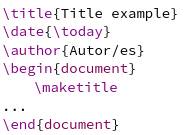
\includegraphics[width=0.5\textwidth]{images/make_title.png}
        \column{0.5\textwidth}
            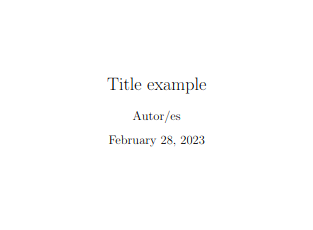
\includegraphics[width=\textwidth]{images/make_title_res.png}
    \end{columns}

    \pause

    \centering
    \textit{O podemos crear la portada mano\ldots{} \textleftarrow\: \textbf{Recomendable}}

\end{frame}